\section{Lezione 4} \hfill 03/03/2026\\
\subsection{Regione costiera}
Il clima è tipicamente mediterraneo:
\begin{itemize}
    \item estati secche e torride;
    \item inverni umidi e miti (raramente la temperatura va sotto 0 \textdegree C).
\end{itemize}
Risulta che esistono diversi fattori limitanti all'adeguata crescita della vegetazione:
\begin{itemize}
    \item principalmente è l'acqua (soprattutto durante l'estate);
    \item il sale, agendo: 
    \begin{enumerate}
        \item nella falda: salando l'acqua, dovuta alla penetrazione del cuneo salino;
        \item in aria: sollevato dai venti, viene trasportato ed a contatto con le foglie le brucia (assorbendo l'umidità e facendole seccare).
    \end{enumerate}
    \item il fuoco, sviluppato in parte dai venti;
    \item i suoli sono facilmente movibili dal vento (salso), essendo principalmente sabbiosi;
    \item le alte temperature favoriscono l'evapotraspirazione;
    \item la forte presenza di animali e dell'uomo (che possono danneggiare le piante), essendo la zona costiera molto abitabile. 
\end{itemize}
I boschi della regione costiera sono importati:
\begin{itemize}
    \item proteggono dal sale le coltivazioni costiere (funz. di protezione);
    \item funzione turistico/ricreativa (seppur limitatamente, data la grande presenza di elementi di fastidio, es. zecche);
    \item funzione paesistica;
    \item funzione produttiva: resina, pinoli, limitata per il legname.
\end{itemize}
L'area immediatamente prospicente al mare è priva di vegetazione data la grande influenza del mare (es. acqua salata, mareggiate, spostamento della sabbia), che non ne permettono la vita.\\
Dove il mare non arriva, si possono notare le prime formazioni di specie erbacee (alofile, ovvero resistenti al sale).\\
Quando queste specie riescono a fissare la duna e fermare la sabbia in movimento, appaiono le specie della gariga: normalmente non superano i 0.5 m di altezza. Non sono presenti tante specie, perchè ancora influenzati dal mare: la più tipica specie è il rosmarino. L'unica funzione della gariga è la protezione.\\
Successivamente avviene la comparsa della macchia: convenzionalmente si suddivide in macchia bassa e macchia alta. In questa formazione avviene un aumento delle specie, sia arbustive che arboree (che mantengono lo stesso il portamento arbustivo).\\
\fbox{ \centering
    \begin{minipage}{0.95\textwidth} 
    Mentre l'arbusto possiede naturalmente più fusti (es. nocciolo), l'albero possiede naturalmente un unico fusto (es. abete).
    \end{minipage}
    }\\
Tendenzialmente, nelle condizioni maggiormente difficili sono presenti le specie pioniere; nella zona marittima sono presenti anche le pioniere (es. ginepri, erica arborea), e successivamente arrivano anche le altre. Le specie presenti nella macchia sono: 
\begin{multicols}{2}
\begin{itemize}
    \item ginepri (es. communis, oxycedrus, coccolone);
    \item erica arborea;
    \item corbezzolo;
    \item mirto comune;
    \item olivastro/olivo;
    \item rosmarino;
    \item alaterno;
    \item cisto (acidofilo, quindi non in ambiente adriatico, tanti in Sardegna e Sicilia);
    \item salicornia;
    \item le ginestre (le mediterranee sono basifile, quelle collinari/dei carbonai sono acidofile);
    \item quercia cocifera (per il colore rosso, tipo Campari);
    \item leccio (in forma arbustiva, date le condizioni difficili);
    \item le lavande;
    \item sommacco.
\end{itemize}
\end{multicols}
\begin{figure}[htbp]
     \centering
     % Prima Immagine
     \begin{subfigure}[b]{0.33\textwidth}
         \centering
         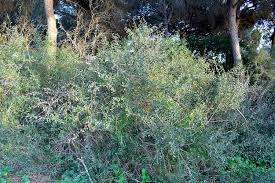
\includegraphics[width=\textwidth]{immagini/alaterno.jpg}
         \caption{Alaterno}
     \end{subfigure}
     \hfill % Spazio elastico tra le immagini
     % Seconda Immagine
     \begin{subfigure}[b]{0.3\textwidth}
         \centering
         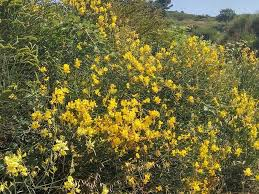
\includegraphics[width=\textwidth]{immagini/ginestre.jpg}
         \caption{Ginestra}
     \end{subfigure}
     \hfill % Spazio elastico tra le immagini
     % Terza Immagine
     \begin{subfigure}[b]{0.3\textwidth}
         \centering
         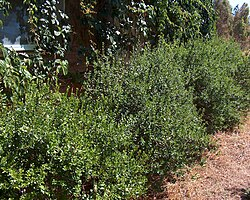
\includegraphics[width=\textwidth]{immagini/mirto_comune.jpg}
         \caption{Mirto}
     \end{subfigure}
     
    % \caption{Didascalia generale del gruppo di immagini.}
     \label{fig:macchia_costiera}
\end{figure}
Essendoci tante specie, la competizione tra gli individui è alta: sono presenti tanti disturbi (e molto diversi): ogni specie è preparata per un proprio disturbo e ciclicamente ne approfittano.\\
I diversi disturbi (e le relative strategie) sono:
\begin{itemize}
    \item il fuoco:
    \begin{enumerate}
        \item pirofitismo attivo: reagisco bene al fuoco (serotinia o capacità pollonifera);
        \item pirofitismo passivo: resistenza al fuoco (cortecce spesse, portamento slanciato).
    \end{enumerate}
    Il passaggio del fuoco permette di mineralizzare la sostanza organica del suolo ed eliminare il soprassuolo vegetato; contemporaneamente apre il cono e fa espellere i semi: una successiva pioggia permette la rinascita della rinnovazione post-incendio. 
    \item i venti salsi: apparati radicali particolari e cuticole delle foglie spesse (in modo che il sale non riesca a penetrare);
    \item la siccità: 
    \begin{enumerate}
        \item sclerofilia delle foglie (foglie molto spesse, con capacità di ridurre la traspirazione, coriacee);
        \item foglie ricoperte di cere (riflesso della radiazione e mantenimento dell'umidità);
        \item periodo vegetativo in inverno e riposo in estate (es.il leccio è capace di fermare il proprio metabolismo quando c'è siccità e riprendere quando inizia a piovere, creando più anelli in un anno);
        \item in certi momenti estremi avviene la caduta delle foglie.
    \end{enumerate}
    \item animali o l'uomo: 
    \begin{enumerate}
        \item aromi strani;
        \item parti spinose.
    \end{enumerate}
\end{itemize}
Tecnicamente, la macchia non è un bosco, perchè non è composto di alberi, ma è formato da arbusti o alberi in forma arbustiva. In Italia, la macchia ricade all'interno delle aree considerate forestate, per motivi economici (fondi per la difesa dagli incendi boschivi).\\
Dal punto di vista selvicolturale, la macchia svolge principalmente la funzione di protezione del suolo: se non ci fosse avverrebbe l'erosione ed il dilavamento delle sostanze nutritive (le piogge sono solitamente battenti, a carattere temporalesco). È fondamentamentale che ci sia la macchia per la protezione del suolo.\\
La macchia è estremamente densa, con una forte copertura e protezione del suolo: sia per quanto riguarda l'erosione/dilavamento e sia per quanto riguarda la temperatura. 
